\chapter{Краткие инструкции по настройке издательской системы \LaTeX}\label{appendix-MikTeX-TexStudio}							% Заголовок
%\addcontentsline{toc}{chapter}{Second call for chapters to participate in the book Machine learning in analysis of biomedical and socio-economic data}	% Добавляем его в оглавление

В SPbPU-BCI-template {\itshape автоматически выставляются необходимые настройки и в исходном тексте шаблона приведены примеры оформления текстово-графических объектов}, поэтому авторам достаточно заполнить имеющийся шаблон текстом главы (статьи), не вдаваясь в детали оформления, описанные далее. Возможный <<быстрый старт>> оформления главы (статьи) под Windows следующий\footnote{Внимание! Пример оформления подстрочной ссылки (сноски).}:

\begin{enumerate}
	\item Установка полной версии TeX Live  \cite{latex-texlive}.  В процессе установки лучше выставить параметр доустановки пакетов <<на лету>>.
	
	\item Установка TexStudio \cite{latex-texstudio}.
	
%		\item установка шрифтов PSCyr для работы с TimesNew\-Roman\-PSMT  	\href{https://github.com/AndreyAkinshin/Russian-Phd-LaTeX-Dissertation-Template/blob/master/PSCyr/Windows.md}{по данной инструкции}. В итоговом документе будет, скорее всего, использован Newton.
	
%	\item Переименование следующих файлов, где вместо \texttt{AuthorsSur\-names} необходимо подставить фамилии авторов (можно сокращать до первых четырех букв): 
%	
%	\begin{enumerate}
%		\item Основной файл \texttt{Book\_title\_ch\_Authors\-Sur\-names.tex}.
%		\item Библиография \texttt{biblio\textbackslash{}Book\_title\_bib\_Authors\-Sur\-na\-mes\-.bib}.
%		\item Пользовательские настройки (при необходимости), \texttt{common\textbackslash{}Book\_\-tit\-le\_ext\_Authors\-Sur\-names.tex}. 
%	\end{enumerate}
%	
%	\item После открытия основного файла \texttt{Book\_title\_ch\_Authors\-Sur\-names.tex} (с новым названием)   переименовать названия по аналогии в следующих командах \texttt{\textbackslash{}input\{\}}:
%	
%	\begin{enumerate}
%		\item \texttt{biblio/Book\_title\_bib\_Authors\-Sur\-names.bib},
%		\item \texttt{common/Book\_title\_ext\_Authors\-Sur\-names.tex (при необходимости) }.
%	\end{enumerate}
%	
	
	\item Запуск TexStudio и компиляция \verb|my_chapter.tex| с помощью команды <<Build\&View>> (например, с помощью двойной зелёной стрелки в верхней панели). {\itshape Иногда, для достижения нужного результата необходимо несколько раз скомпилировать документ.}
	
	\item В случае, если не отобразилась библиография, можно
	
	\begin{itemize}
		\item воспользоваться командой Tools $\to$ Commands $\to$ Biber, затем запустив Build\&View;
		
		\item настроить автоматическое включение библиографии в настройках Options $\to$ Configure TexStudio $\to$ Build $\to$  Build\&View (оставить по умолчанию, если сборка происходит слишком долго): \texttt{txs:///pdflatex | txs:///biber | txs:///pdflatex | txs:///pdflatex | txs:///\-view-pdf}.
	\end{itemize}
	
\end{enumerate}

В случае возникновения ошибок, попробуйте скомпилировать документ до последних действий или внимательно ознакомьтесь с описанием проблемы в log-файле. Бывает полезным переход (по подсказке TexStudio) в нужную строку в pdf-файле или запрос с текстом ошибке в поисковиках. Наиболее вероятной проблемой при первой компиляции может быть отсутствие какого-либо установленного пакета \LaTeX. 

В случае корректной работы настройки <<установка на лету>> все дополнительные пакеты будут скачиваться и устанавливаться в автоматическом режиме. Если доустановка пакетов осуществляется медленно (несколько пакетов за один запуск компилятора), то можно попробовать установить их в ручном режиме следующим образом:

\begin{enumerate}[1.]
	\item Запустите программу: меню $\to$ все программы $\to$ MikTeX $\to$ Maintenance (Admin) $\to$ MiKTeX Package Manager (Admin).
	\item Пользуясь поиском, убедитесь, что нужный пакет присутствует, но не установлен (если пакет отсутствует воспользуйтесь сначала MiKTeX Update (Admin)).
	\item Выделив строку с пакетом (возможно выбрать несколько или вообще все неустановленные пакеты), выполните установку Tools $\to$ Install или с помощью контекстного меню.
	\item После завершения установки запустите программу MiKTeX Settings (Admin).
	\item Обновите базу данных имен файлов Refresh FNDB.
\end{enumerate}


Для проверки текста статьи на русском языке полезно также воспользоваться настройками Options $\to$ Configure TexStudio $\to$ Language Checking $\to$  Default Language. Если русский язык <<ru\_RU>> не будет доступен в меню выбора, то необходимо вначале выполнить Import Dictionary, скачав из интернета любой русскоязычный словарь. 


%\chapter{\normalfont\normalsize{}Часто задаваемые вопросы (FAQ)}\label{Appendix-FAQ}							% Заголовок
%%\addcontentsline{toc}{chapter}{Second call for chapters to participate in the book Machine learning in analysis of biomedical and socio-economic data}	% Добавляем его в оглавление


Далее приведены формулы \eqref{eq:Pi-app2}, \eqref{eq:Pi-app2-},  \firef{fig:spbpu_hydrotower-app2}, \firef{fig:spbpu_hydrotower-app2-}, \taref{tab:ToyCompare-app2}, \taref{tab:ToyCompare-app2-}.


\begin{equation}% лучше не оставлять пропущенную строку (\par) перед окружениями для избежания лишних отсупов в pdf
\label{eq:Pi-app2-} % eq - equations, далее название, ch поставлено для избежания дублирования
\pi \approx 3,141.
\end{equation}

%
\begin{figure}[ht!] 
	\center
	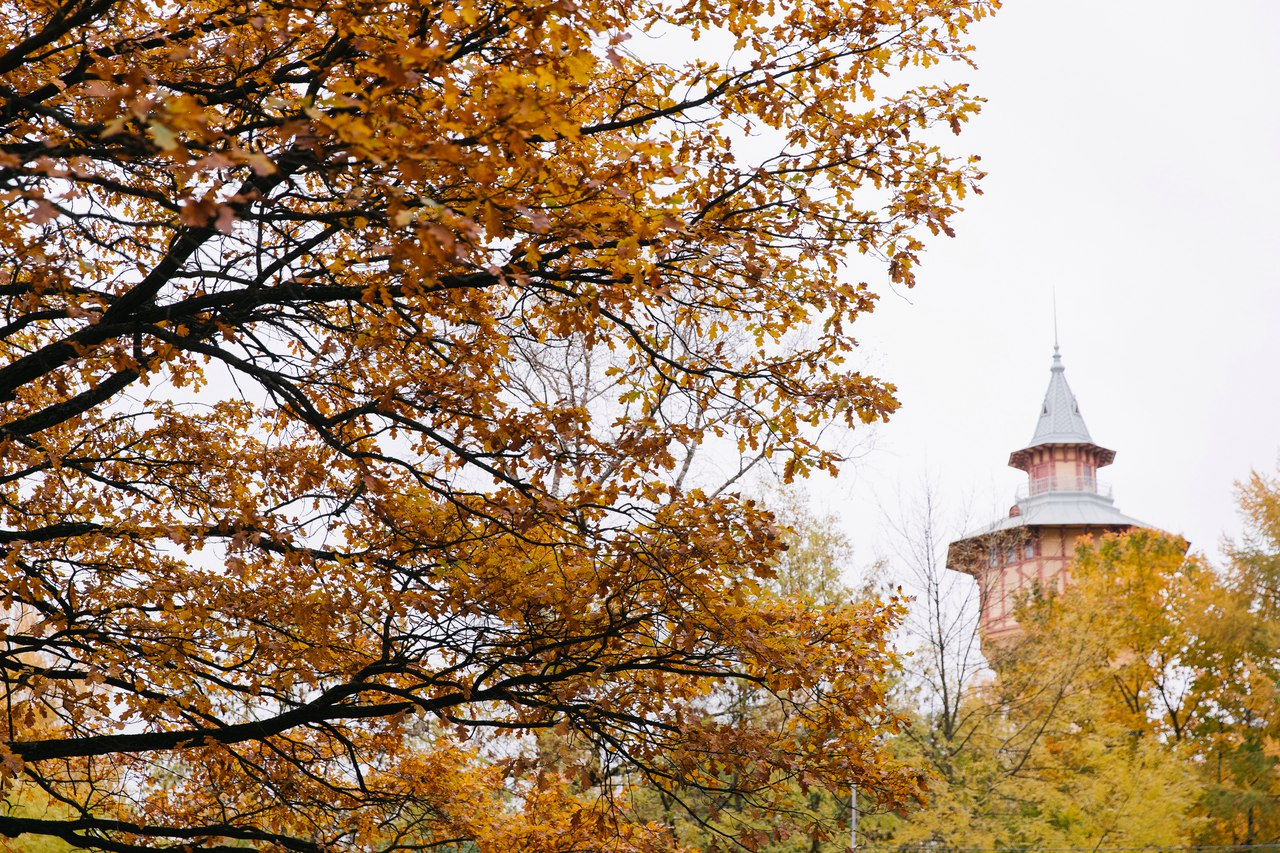
\includegraphics [scale=0.27] {my_folder/images//spbpu_hydrotower}
	\caption{Вид на гидробашню СПбПУ \cite{spbpu-gallery}} 
	\label{fig:spbpu_hydrotower-app2-}  
\end{figure}

\begin{table} [htbp]% Пример оформления таблицы
	\centering\small
	\caption{Представление данных для сквозного примера по ВКР \cite{Peskov2004}}%
	\label{tab:ToyCompare-app2-}		
	\begin{tabular}{|l|l|l|l|l|l|}
		\hline
		$G$&$m_1$&$m_2$&$m_3$&$m_4$&$K$\\
		\hline
		$g_1$&0&1&1&0&1\\ \hline
		$g_2$&1&2&0&1&1\\ \hline
		$g_3$&0&1&0&1&1\\ \hline
		$g_4$&1&2&1&0&2\\ \hline
		$g_5$&1&1&0&1&2\\ \hline
		$g_6$&1&1&1&2&2\\ \hline		
	\end{tabular}	
	\normalsize% возвращаем шрифт к нормальному
\end{table}




\section{Параграф приложения}\label{app-2-1}							


\subsection{Название подпараграфа} \label{ch2:subsec-title-abbr} %название по-русски


Название подпараграфа оформляется с помощью команды  \texttt{\textbackslash{}subsection\{...\}}.

Использование подподпараграфов в основной части крайне не рекомендуется.
\subsubsection{Название подподпараграфа}\label{ch2:subsubsec-title-abbr} %название по-русски

\begin{equation}% лучше не оставлять пропущенную строку (\par) перед окружениями для избежания лишних отсупов в pdf
\label{eq:Pi-app2} % eq - equations, далее название, ch поставлено для избежания дублирования
\pi \approx 3,141.
\end{equation}
%
%
\begin{figure}[ht!] 
	\center
	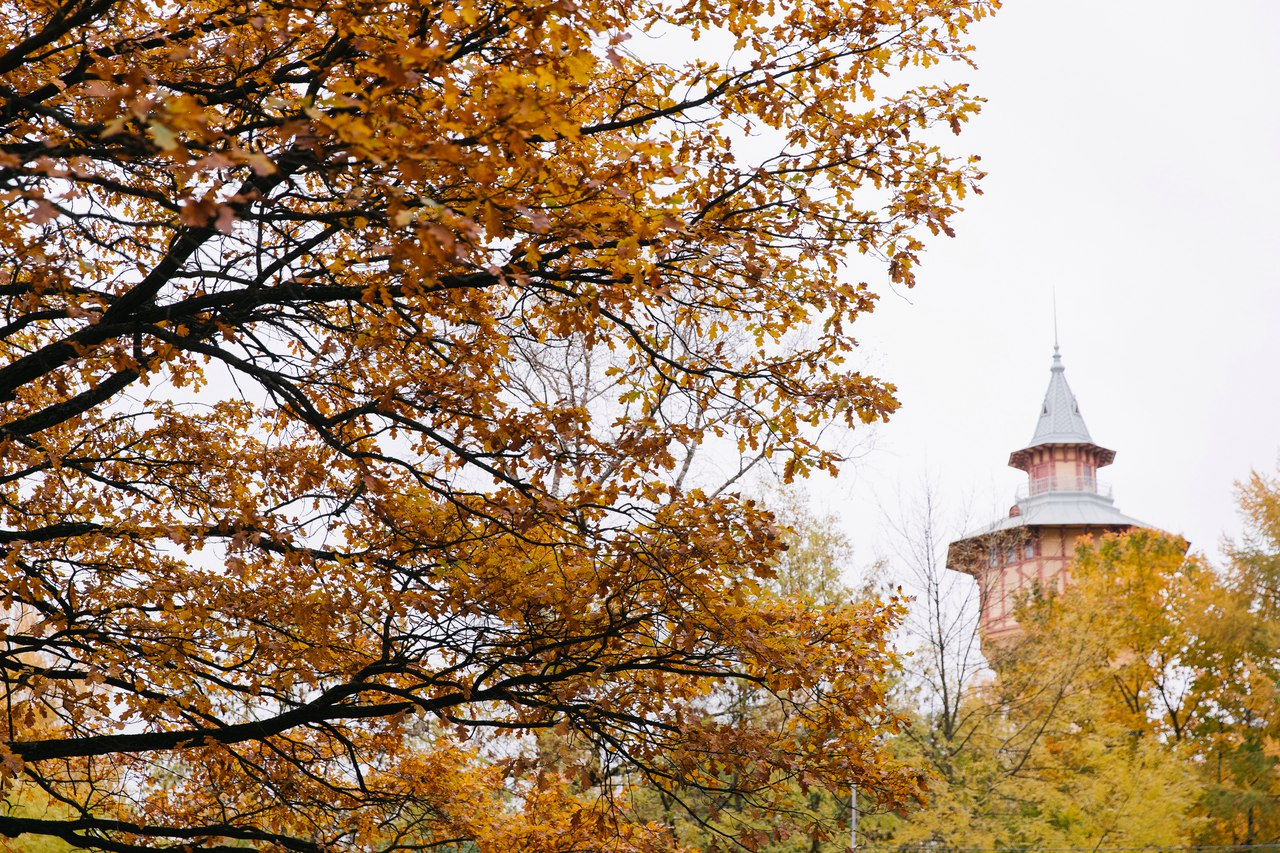
\includegraphics [scale=0.27] {my_folder/images//spbpu_hydrotower}
	\caption{Вид на гидробашню СПбПУ \cite{spbpu-gallery}} 
	\label{fig:spbpu_hydrotower-app2}  
\end{figure}
%




\begin{table}[t!]% Пример оформления таблицы
	\centering\small
	\caption{Представление данных для сквозного примера по ВКР \cite{Peskov2004}}%
	\label{tab:ToyCompare-app2}		
	\begin{tabular}{|l|l|l|l|l|l|}
		\hline
		$G$&$m_1$&$m_2$&$m_3$&$m_4$&$K$\\
		\hline
		$g_1$&0&1&1&0&1\\ \hline
		$g_2$&1&2&0&1&1\\ \hline
		$g_3$&0&1&0&1&1\\ \hline
		$g_4$&1&2&1&0&2\\ \hline
		$g_5$&1&1&0&1&2\\ \hline
		$g_6$&1&1&1&2&2\\ \hline		
	\end{tabular}	
	\normalsize% возвращаем шрифт к нормальному
\end{table}


%% В случае, когда таблица (рисунок) размещаются на последней странице, для переноса названия приложения на новую строку используем:
\NewPage % начать новое приложение с новой страницы 